\section{Benchmarks}
\label{sec:benchmarks}
We ran various experiments to compare the different variants of the
algorithm C2 between themselves and to the other algorithms. All the
experiments were run on four dual-core Intel Xeon E5430 (2.6GHz),
eventually using the parallelised version of the algorithm.

\begin{figure}
  \centering
%  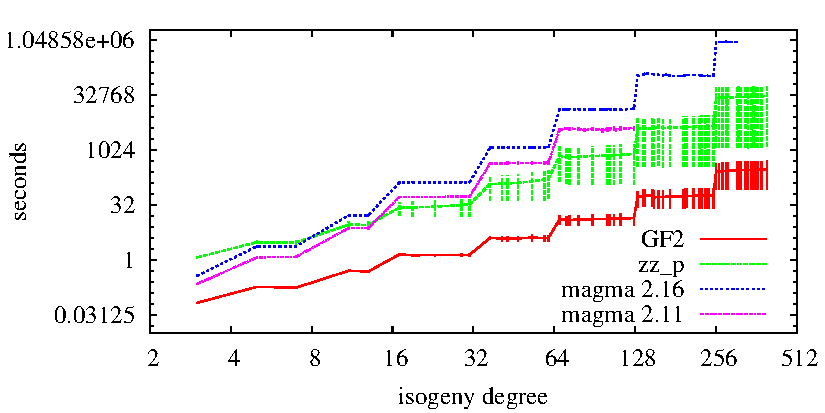
\includegraphics[width=0.9\textwidth]{p2}
  \caption{Comparative timings for different implementations of C2-AS-FI-MC with curves defined over $\F_{2^{101}}$. Plot in logarithmic scale.}
  \label{fig:2-101}
\end{figure}

The first set of experiments was run to evaluate the benefits of using
the fast algorithms in~\cite{DFS09}. We selected pairs of isogenous
curves over $\F_{2^{101}}$ such that the height of the tower is
maximal (observe that this is always the case for cryptographic
curves). The library \texttt{FAAST} offers two types for finite field
arithmetics in characteristic $2$: \texttt{zz\_p} which is a generic
type for word-precision $p$ and \texttt{GF2} which uses the optimised
algorithms of the library \texttt{gf2x}. We compared implementations
of C2-AS-FI-MC using these two types with an implementation written in
Magma. The results are in figure~\ref{fig:2-101}: we plot a line for
the average running time of the algorithm and bars around it for
minimum and maximum execution times of the final loop. Besides the
dramatic speedup obtained by using the ad-hoc type \texttt{GF2}, the
algorithmic improvements of \texttt{FAAST} over Magma are evident as
even \texttt{zz\_p} is one order of magnitude faster.

\begin{table}
  \centering
  \begin{tabular}{r r r r r r r r}
    \hline
    $\ell$ & $E[p^k]$ & $E'[p^k]$ & FI & RFR & MC & Avg tries & Avg loop time\\
    \hline
    31 & 1.3128 & 1.3128 & 1.1058 & 0.00218 & 0.00218 & 64 & 0.279\\
    61 & 3.5454 & 3.5464 & 2.5236 & 0.00783 & 0.00900 & 128 & 2.154 \\
    127 & 9.2975 & 9.3026 & 5.6881 & 0.03147 & 0.03634 & 256 & 17.359 \\
    251	& 23.7984 & 23.7984 & 12.7251 & 0.12415 & 0.14519 & 512 & 137.902 \\
    397 & 59.7439 & 59.7579 & 28.3387 & 0.36822 & 0.58027 & 1024 & 971.254 \\
    \hline
  \end{tabular}
  \caption{Comparative timings for the phases of C2-AS-FI-MC for curves over $\F_{2^{101}}$.}
  \label{tab:C2}
\end{table}

Table~\ref{tab:C2} shows detailed timings for each phase of
C2-AS-FI-MC. The column FI reports the time for one interpolation, the
column MC the time for one modular composition; comparing these two
columns the gain from passing from C2-AS-FI to C2-AS-FI-MC is
evident. Columns RFR (rational fraction reconstruction) and MC
constitute the Cauchy interpolation step that is repeated in the final
loop. The last column reports the average time spent in the loop: it
is by far the most expensive phase and this justifies the attention we
paid to FI and MC; only on some huge examples we approached the
crosspoint between these two algorithms.

\begin{figure}
  \centering
%  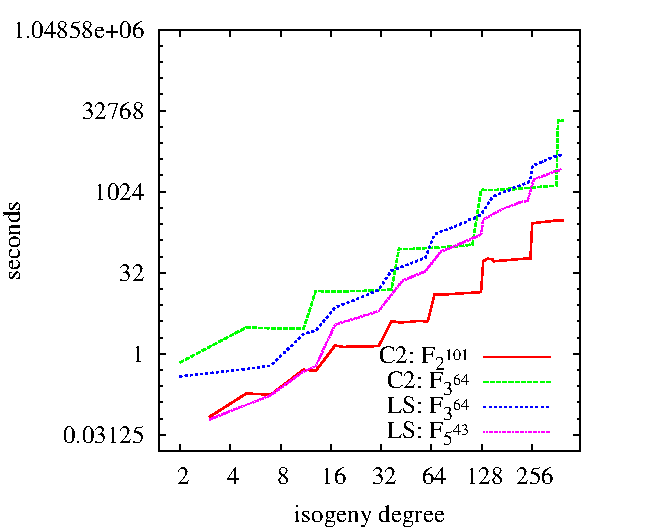
\includegraphics[height=0.45\textwidth]{C2-LS}
%   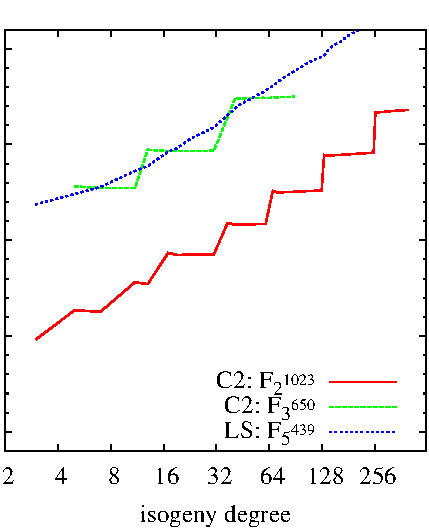
\includegraphics[height=0.45\textwidth]{C2-LS2}
   \caption{Comparative timings for C2-AS-FI-MC (C2) and LS over
     different curves. Plot in logarithmic scale.}
  \label{fig:comp}
\end{figure}

Next, we compare the running times of C2-AS-FI-MC and LS over curves
of half the cryptographic size in figure~\ref{fig:comp} (left). We
only plot average times for C2, in characteristic $2$ we only plot the
timings for \texttt{GF2}. From the plot it is clear that C2-AS-FI-MC
only performs better than LS for $p=2$, but in this case the algorithm
of~\cite{Ler96} is by far better.  Figure~\ref{fig:comp} (right) shows
that LS slowly gets worse than C2, however comparing a Magma prototype
to our highly optimised implementation of C2-AS-FI-MC is somewhat
unfair and probably the crosspoint between the two algorithms lies
much further. Furthermore, it is unlikely that C2-AS-FI-MC could be
practical for any $p>3$ because of its high dependence on $p$, while
LS scales pretty well with the characteristic as shown in
figure~\ref{fig:LSp}.

\begin{figure}
  \centering
%  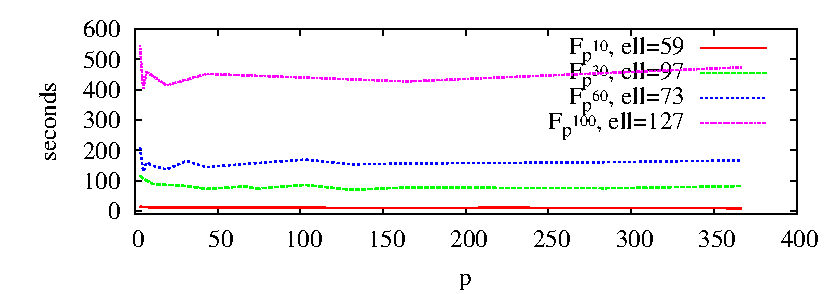
\includegraphics[width=0.9\textwidth]{LSp}
  \caption{Timings for LS for different fields. We increase
    $p$ while taking constant $d$ and the isogeny degree.}
  \label{fig:LSp}
\end{figure}

We can hardly hide our disappointment concluding that, despite their
good asymptotic behaviour and our hard work implementing them, the
variants derived from C2 don't seem to have any practical application,
at least for present data sizes. We hope that in the future the
algorithms presented here may turn useful to compute very large data
that are currently out of reach.




% Local Variables:
% mode:flyspell
% ispell-local-dictionary:"british"
% TeX-master: "ec-isogeny"
% End:
%
% LocalWords:  Schreier Artin pseudotrace frobenius bivariate Joux Sirvent FFT
% LocalWords:  Couveignes isogenies Schoof isogeny cryptosystems Lercier
% LocalWords:  precomputation arithmetics polylogarithmic Karatsuba precomputes
% LocalWords:  endomorphisms  isogenous
